\chapter{Il sistema M-NAT: un approccio integrato per la predizione acustica e navale}

Il progetto \textbf{M-NAT} rappresenta un'iniziativa di ricerca avanzata che combina la modellazione acustica sottomarina con algoritmi di intelligenza artificiale, includendo il monitoraggio e la predizione del comportamento navale al fine di una modellazione più accurata.

M-NAT innova integrando modellazione fisica e tecniche \textit{data-driven} all'interno di un framework scalabile e configurabile. La combinazione di BellHop e TrAISformer offre uno strumento per applicazioni marine, monitoraggio ambientale e \textit{intelligence} navale.

\section{Componenti principali}

\subsection{Modellazione acustica sottomarina}

Il sistema si basa su \textbf{BellHop}, un programma di ray-tracing acustico estremamente affidabile, originariamente sviluppato in FORTRAN per simulazioni di campo acustico in oceano \cite{porter2011bellhop,long2012bellhop}. BellHop è stato ampiamente adottato con interfacce Python, per facilitare integrazioni nei workflow moderni \cite{fang2024bellhop}. In M-NAT, BellHop gestisce sorgenti acustiche come navi e \textit{airgun}, modellando la propagazione sonora tenendo conto della batimetria (mappatura delle profondità marine), profili di velocità del suono e linee costiere.

\subsection{Predizione delle traiettorie navali}

Il componente \textit{AIS} si fonda sul modello \textbf{TrAISformer}, un \textit{transformer} generativo adattato alla predizione delle traiettorie navali da dati AIS \cite{nguyen2021traisformer}. 

L'AIS, acronimo di \textit{Automatic Identification System}, è un sistema che permette alle imbarcazioni di identificarsi reciprocamente e di scambiare dati cruciali con altre navi, stazioni terrestri e centri di controllo del traffico costiero.

\noindent Il modello:
\begin{itemize}
  \item codifica latitudine, longitudine, velocità e rotta in \textit{embedding} separati;
  \item utilizza una \textit{loss} a base di entropia incrociata per gestire la natura multimodale dei dati;
  \item sfrutta l'architettura \textit{transformer} per estrarre dipendenze temporali a medio-lungo termine \cite{nguyen2021traisformer}.
\end{itemize}

\section{Tecnologie e performance}

La struttura modulare del progetto consente:
\begin{itemize}
  \item parametrizzazione completa via configurazione JSON (frequenze, profondità, risoluzioni);
  \item compatibilità con strumenti esterni grazie a input multidimensionali (NetCDF, HDF5).
\end{itemize}

Il progetto M‑NAT si fonda su un ecosistema tecnologico moderno e consolidato, che garantisce flessibilità, prestazioni e scalabilità:

\begin{itemize}
  \item \textbf{PyTorch, NumPy e SciPy} per il calcolo numerico e il \textit{machine learning}. 
    NumPy costituisce la base per l'elaborazione efficiente di array N‑dimensionali, permettendo operazioni di algebra lineare, trasformate e indicizzazione avanzate \cite{walt2011numpy}. SciPy amplia le capacità di NumPy con moduli specializzati nell'ottimizzazione, nell'interpolazione, nell'elaborazione di segnali e solutori ODE \cite{virtanen2020scipy}. PyTorch, infine, fornisce un framework GPU‑accelerato per la computazione tensoriale e l'apprendimento profondo, con supporto ad autograd e modelli neurali dinamici \cite{paszke2019pytorch}.

  \item \textbf{GeoPandas, GDAL e Shapely} per le elaborazioni geospaziali. Pandas è una delle librerie più importanti e utilizzate per la manipolazione e l'analisi dei dati. È uno strumento open-source, veloce, flessibile ed espressivo, costruito sul linguaggio di programmazione Python; GeoPandas estende Pandas per gestire dati geografici tramite GeoDataFrame, integrando funzionalità di Shapely per operazioni geometriche e GDAL/PROJ per lettura, scrittura e trasformazioni dei sistemi di coordinate \cite{geopandas2025}. Questo consente di effettuare analisi complesse come intersezioni, \textit{buffering}, \textit{overlay} e calcolo di aree in modo efficiente.

  \item \textbf{Xarray, NetCDF4 e HDF5} per la gestione di dati ambientali multidimensionali. Queste librerie permettono la lettura/scrittura di formati standard come NetCDF e HDF5, fondamentali quando si lavora con dati oceanografici quali profili di velocità del suono, batimetria e mappe \textit{raster}.

  \item \textbf{Numba e accelerazione GPU} per ottimizzare le prestazioni. Numba permette di compilare al volo porzioni di codice Python in codice macchina ottimizzato, riducendo significativamente i tempi di calcolo numerico. L'uso di GPU permette di accelerare sia PyTorch sia librerie compatibili come CuPy, estendendo l'efficienza alle operazioni massivamente parallele.
\end{itemize}

Insieme, queste tecnologie offrono una suite completa per acquisire e processare grandi quantità di dati scientifici e ambientali, permettendo di addestrare e ottimizzare modelli neurali complessi per la previsione di traiettorie. Così facendo è possibile eseguire elaborazioni geospaziali e garantire alte prestazioni su CPU e GPU con \textit{workflow} paralleli e modulari.

\section{Applicazioni e impatto}

M-NAT è fruibile in scenari operativi come:
\begin{itemize}
  \item valutazione del rumore antropico in ambiente marino;
  \item pianificazione di rotte minimizzanti il disturbo acustico;
  \item supporto alla trasmissione di dati utilizzando acque marine/oceaniche.
\end{itemize}

\section{Il Modello \textit{\textit{airgun}NoiseEstimation}}

Il modello \textbf{\textit{airgun}NoiseEstimation} simula la propagazione del rumore generato da un \textit{\textit{airgun}} sottomarino e produce una mappa dell'inquinamento acustico marino nella zona di studio.

L'obiettivo del modello è stimare come il rumore emesso da un \textit{\textit{airgun}}, ossia una sorgente impulsiva ad alta potenza usata nelle prospezioni sismiche, si propaghi nell'ambiente marino, producendo una mappa spaziale dei livelli sonori (in dB) attorno alla sorgente.

\subsection{Fasi del processo di simulazione}

\begin{enumerate}
  \item \textbf{Definizione dell'area di studio}, tipicamente un cerchio centrato sull'\textit{\textit{airgun}} con raggio prestabilito (es. 1000 km).
  \item \textbf{Suddivisione in settori radiali}: l'area viene suddivisa in \(N\) spicchi (es. 90) per valutare radialmente la propagazione.
  \item \textbf{Simulazione della propagazione lungo ciascun settore}, considerando:
    \begin{itemize}
      \item batimetria e morfologia del fondale;
      \item rotte navali che possono influenzare la diffusione;
      \item profili di velocità del suono (\textit{sound speed profiles});
      \item ostacoli naturali come coste e isole.
    \end{itemize}
  \item \textbf{Calcolo dei livelli di rumore} lungo ogni linea radiale, in \(\mathrm{dB_{SPL}}\). Questa unità di misura rappresenta il livello di pressione sonora. È una misura logaritmica della pressione acustica relativa a un valore di riferimento, usato per quantificare l'intensità del suono. \cite{db-spl-definition}
  \item \textbf{Assemblaggio della mappa finale}, combinando tutti i settori in un dataset \textit{geoposizionato}.
\end{enumerate}

\subsection{Output generati}

Il modello produce un file contenente coordinate GPS, livelli di pressione sonora e informazioni ambientali. In particolare, i dati presenti sono i seguenti:

\begin{itemize}
  \item coordinate GPS dei punti campionati;
  \item livelli di rumore in dB riferiti a 1 microPascal $(\mu Pa)$ a 1 metro dalla sorgente acustica;
  \item dati ambientali (profondità, distanza dalla sorgente);
  \item etichette di settore per ogni punto.
\end{itemize}

Questi dati possono essere elaborati ulteriormente con il fine di visualizzare i dati contenuti sotto forma di rappresentazioni grafiche significative. Il contributo al progetto si è focalizzato su quest'ultimo aspetto, ossia rappresentare decine di migliaia di \textit{datapoints} su una mappa digitale, permettendo un'interazione dinamica. Si veda un esempio di rappresentazione grafica in Figura \ref{fig:preview-heatmap}.

\begin{figure}
    \centering
    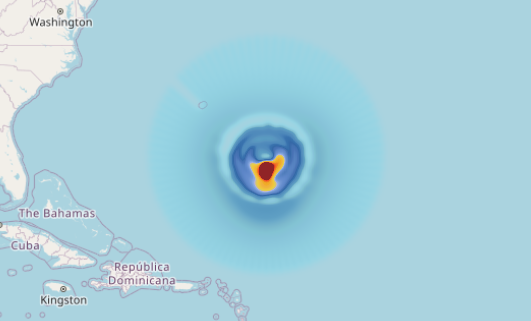
\includegraphics[width=0.75\linewidth]{images/heatmap.png}
    \caption{Visualizzazione dei dati generati su mappa (HeatMap)}
    \label{fig:preview-heatmap}
\end{figure}

Una breve anteprima dei dati testuali generati:

\begin{table}[ht]
\centering
\label{tab:data}
\begin{tabular}{
    S[table-format=2.15]
    S[table-format=-2.1]
    S[table-format=2.15]
    S[table-format=4.0]
    S[table-format=4.15]
    S[table-format=1.1]
}
\toprule
{Latitude} & {Longitude} & {Value} & {Bathy1} & {Bathy2} & {Sector} \\
\midrule
37.25897980148502 & -59.3 & 88.04606789424417 & 1003 & 5163.03076171875  & 0.0 \\
37.24995686563234 & -59.3 & 88.04978137920247 & 2007 & 5167.09033203125  & 0.0 \\
37.24093392977967 & -59.3 & 88.05349035487939 & 3011 & 5166.5244140625   & 0.0 \\
37.231910993927   & -59.3 & 88.05719509329765 & 4015 & 5166.5576171875   & 0.0 \\
37.22288805807432 & -59.3 & 88.06089653237328 & 5019 & 5166.21142578125  & 0.0 \\
37.21386512222165 & -59.3 & 88.06459277272671 & 6022 & 5161.037109375    & 0.0 \\
37.20484218636896 & -59.3 & 88.06828474014407 & 7026 & 5158.3720703125   & 0.0 \\
\bottomrule
\end{tabular}
\end{table}

\subsection{Utilità principale}

I risultati generati dal modello permettono di stimare con precisione le aree di maggiore impatto acustico attorno alla sorgente, evidenziando come il rumore si attenui con la distanza seguendo le leggi della propagazione sott'acqua. \cite{airgun_marine_life} 
Grazie all'inclusione di rotte navali e dettagli morfologici come isole, coste e batimetria, il modello è in grado di identificare sia zone con un livello di rumore più elevato, sia zone \say{d'ombra} dove il suono risulta attenuato rispetto all'ambiente circostante.

\noindent In sintesi, il modello trasforma una simulazione fisica complessa in un output geografico e operativo, utile per la gestione responsabile dell'inquinamento acustico marino.
